\documentclass{article}
\usepackage[utf8]{inputenc}
\usepackage{amsmath}
\usepackage{graphicx}
\usepackage{listings}
\usepackage{xcolor}
\usepackage{geometry}
\geometry{margin=1in}

\definecolor{codegreen}{rgb}{0,0.6,0}
\definecolor{codegray}{rgb}{0.5,0.5,0.5}
\definecolor{codepurple}{rgb}{0.58,0,0.82}
\definecolor{backcolour}{rgb}{0.95,0.95,0.92}

\lstdefinestyle{mystyle}{
    backgroundcolor=\color{backcolour},
    commentstyle=\color{codegreen},
    keywordstyle=\color{magenta},
    numberstyle=\tiny\color{codegray},
    stringstyle=\color{codepurple},
    basicstyle=\ttfamily\footnotesize,
    breakatwhitespace=false,
    breaklines=true,
    captionpos=b,
    keepspaces=true,
    numbers=left,
    numbersep=5pt,
    showspaces=false,
    showstringspaces=false,
    showtabs=false,
    tabsize=2
}
\lstset{style=mystyle}

\begin{document}

\title{Mini Project 3}
\author{EECE 7398 Legged Robotics}
\date{}
\maketitle

\section*{Code Listing}

\subsection*{\texttt{func\_zero\_dynamics.m}}
\begin{lstlisting}[language=Matlab]
% Simulation zero dynamics of 3 link biped in the sagittal plane
%
% Inputs:
%       t: time
%       z: cyclic variables [q1, dq1]
%       a: bezier coefficient for q2 - a(1:5), and q3 - a(6:10)
%       s_params: [z_min, z_max] - max and min angles in gait
%       
% Outputs:       
%       dz = [dq1, ddq1]
%
function dz = func_zero_dynamics(t,z,a,s_params)

z_min = s_params(1); 
z_max = s_params(2); 
delq = z_max - z_min;

q1 = z(1); dq1 = z(2);

% Computes gait timing variable s
% 
% Inputs: 
%       q1: cyclic variable
%       q1_min: minimum value for q1 during gait
%       q1_max: max value for gait
%
% Output: 
%       s: gait timing variable
%
s = func_gait_timing(q1,z_min,z_max);
if s > 1;     s = 1;
elseif s < 0; s = 0;
end

alpha2 = a(1:5);
alpha3 = a(6:10);

% find based on s and bezier definition
q2 = bezier(s, 4, alpha2);
q3 = bezier(s, 4, alpha3);
db_ds2 = d_ds_bezier(s, 4, alpha2);
db_ds3 = d_ds_bezier(s, 4, alpha3); 

dq2 = db_ds2 * (dq1/delq);
dq3 = db_ds3 * (dq1/delq);

q = [q1, q2, q3];
dq = [dq1, dq2, dq3];

% Get model paramters
[r,m,Mh,Mt,l,g] = func_model_params;
params = [r,m,Mh,Mt,l,g];

% Compute D,C,G,B matrices
% Inputs:
%       q
%       dq
%       params
%
% Output: [D,C,G,B]
%
[D,C,G,~] = func_compute_D_C_G_B(q,dq,params);


%%%%%%%%%%%%%%%%%% Apply dynamics partitioning to compute the zero dynamics
%%%%%%%%%%%%%%%%%% equations %%%%%%%%%%%%%%%%%%%%%%%%%%%%%%%%%%%%%%%%%%%%%%

% E.g., 
D1 = D(1, 1);
D2 = D(1, 2:3);
H1 = C(1,:)*dq' + G(1);

%------------------------------------------------------------------------%

% Get beta1 term to compute dz
%
% Inputs: s, [dq1, delq], [alpha2, alpha3]
%       s: gait timing variable
%       dq1: velocity of cyclic variable = z2
%       delq: difference between z_max and z_min in s, needed when
%               computing db/ds
%       alpha2: Bezier coefficient (1st to 5th) for q2
%       alpha3: Bezier coefficient (1st to 5th) for q3
%
% Output:
%       beta1: one of 2 matrices obtained when computing ddq_b (acceleration
%               of body coordinates) 
%       	y = h(x) = q_b - b(s), when y = 0,  q_b = b(s)
%           taking two time derivatives we get:
%       	ddq_b = d/ds(db(s)/ds*ds/dt)*ds/dt + db(s)/ds * d^2(s)/dt^2
%                 = beta1 + beta2*ddq_1
%           Note: d^2(s)/dt^2 = 1/delq*d^2(q1)/dt^2
%
%       	beta1 = d/ds(db(s)/ds*ds/dt)*ds/dt
%        	beta2 = db(s)/ds*1/delq
%
beta1 = func_compute_beta1(s, [dq1, delq], [alpha2, alpha3]);

% Compute 1st partial derivative of Bezier polynomial
% Inputs:
%       s: gait timing variable
%       M: order of Bezier polynomial, in this case 4th order
%       alpha: Coefficients for the polynomial, need M+1
%
% Outputs:
%       db/ds
%

beta2 = [db_ds2; db_ds3]/delq;

%------------------------------------------------------------------------%

dz(1) = z(2);
dz(2) = (-H1 - D2*beta1) / (D1 + D2*beta2);

dz = [dz(1), dz(2)]';
end
\end{lstlisting}

\subsection*{\texttt{Optimize.m}}
\begin{lstlisting}[language=Matlab]
% Optimize intial conditions for ZD states and Bezier coeffs using fmincon
%
% Zero dynamics simulator takes pre-impact condition so that should be I.C.
% for fmincon as well

%------------------------------------------------------------------------%

%[q1, dq1] pre impact conditions - last known working solution (old Bezier)
z_minus = [-0.3407, -2.6352];

% Bezier coefficients - last known working solution
alpha = [0.4553, 0.6698, 0.8463];   %for q2 - alpha 3rd - 5th
gamma = [2.4988, 2.6419, 2.8039];   %for q3 - alpha 3rd - 5th


%   f0 = [q10, dq10, alpha(3-5)_q2, alpha(3-5)_q3]
%       q10: pre-impact inital angle for q1
%       dq10: pre-impact inital velocity for dq1
%       alpha(3-5)_q2:
%                   3rd to 5th Bezier coefficient for q2
%       alpha(3-5)_q3:
%                   3rd to 5th Bezier coefficient for q3
%
f0 = [z_minus, alpha, gamma];   %parameters that need to be optimized

%------------------------------------------------------------------------%

% Lower and upper bounds for optimizer - [q1 q1_dot, alpha q2, alpha q3]
%
% epsilon for angles
eps = 0.15;
% epsilon for velocity
eps_v = 0.5;
lb = [z_minus(1)-eps, z_minus(2)-eps_v, alpha-eps, gamma-eps];
ub = [z_minus(1)+eps, z_minus(2)+eps_v, alpha+eps, gamma+eps];

%------------------------------------------------------------------------%

%%%% Run optimizer

opts = optimoptions('fmincon','Algorithm','interior-point',...
                    'MaxIterations',1000,...
                    'StepTolerance',1e-6,...
                    'FunctionTolerance',1e-2);
opts.Display = 'iter';
opts.EnableFeasibilityMode = true;
opts.SubproblemAlgorithm = 'cg';


% using only bounds and nonlinear contraints
%
% Outputs: f - optimized parameters [qt, dqt, qt_LR_max, alphaR, alphaL]
%          J - Cost to minimize
%
[f, J] = fmincon(@(f) pass_cost_ZD(f), f0, [],[],[],[], lb,ub, @confuneq,opts);

disp('solution found!');

f

% ---- PRINT: final solution summary ----
fprintf('\n=== Final Solution ===\n');
fprintf('f   = [%.4f, %.4f, %.4f, %.4f, %.4f, %.4f, %.4f, %.4f]\n', f);
fprintf('Cost J = %.6f\n', J);
alpha2_full = [-f(5), -f(4), f(3:5)];
[r,~,~,~,~,~] = func_model_params;
q1_preimpact = f(1); q2_preimpact = alpha2_full(5);
step_length = abs(r*sin(q1_preimpact) + r*sin(q1_preimpact - q2_preimpact));
fprintf('Step length = %.4f m\n', step_length);
% ---- END PRINT ----

% Function only exists to pass cost as a scalar output for fmincon, actual
% cost calculation happends in func_cost_ZD
%
function J = pass_cost_ZD(y)

[J, ~] = func_cost_ZD(y);

end

%------------------------------------------------------------------------%

% Simulate a single step of zero dynamics and get cost
%
% Inputs: [z_plus, a, s_params]
%       z_plus: [q1, dq1] post impact condition
%       a: [alpha2, alpha3] Bezier coefficients for q2 and q3
%       s_params: [q1_min, q1_max]
%
% Outputs: [J, z_sol]
%       J: Cost
%       z_sol: solution to zero dynamics ODE45
%
function [J, z_sol] = func_cost_ZD(f)

%%%% Simulate

% Simulation of a single step of ZD to using preimpact conditions
%   applies impact first then simulates zero dynamics
%
% Inputs: f = [q10, dq10, alpha(3-5)_q2, alpha(3-5)_q3]
%       q10: pre-impact inital angle for q1
%       dq10: pre-impact inital velocity for dq1
%       alpha(3-5)_q2:
%                   3rd to 5th Bezier coefficient for q2
%       alpha(3-5)_q3:
%                   3rd to 5th Bezier coefficient for q3
%
% Outputs:
%       t_sol - time (s) of zero dynamics
%       z_sol - [q1, dq1] post impact dynamics
%
[t_sol, z_sol] = sim_zero_dynamics(f);

%%%% Compute cost

% Variables needed to compute control action
% Match sim_zero_dynamics convention: q1_min=-f(1)=+0.3065 (post-impact,
% start of swing), q1_max=f(1)=-0.3065 (pre-impact, end of swing).
% This ensures s = (q1 - q1_min)/(q1_max - q1_min) runs 0->1 through z_sol.
q1_min = -f(1);
q1_max =  f(1);

s_params = [q1_min, q1_max];

alpha2 = [-f(5), -f(4), f(3:5)];
alpha3 = [f(8)-f(5), -f(7)+2*f(6), f(6:8)];

a = [alpha2, alpha3];

J = 0;
for i = 1:length(t_sol)
    % Post compute control action
    %
    % Inputs: [z, a, s_params]
    %       z: [q1, dq1]
    %       a: [alpha2, alpha3] - 1st to 5th Bezier coefficient for q2 and q3
    %       s_params: [q1_min, q1_max]
    %
    % Output:
    %       u: control action
    %
    u = func_compute_control_action(z_sol(i,:),a,s_params);
    
    % Cost = sum of norms of control action
    J = J + norm(u)^2;
end
% Normalize after loop
J = J / length(t_sol);


end

%------------------------------------------------------------------------%

% Nonlinear constraint for optimizer
%
% Inputs: f: [q1, dq1, alpha2(3:5), alpha3(3:5)]
%
% Output: [c, ceq]
%       c: nonlinear inequality contraint
%       ceq: nonlinear equality contraint
%
function [c,ceq] = confuneq(f)

z_i = f(1:2);       %Pre-impact states

% Simulation of a single step of ZD to using preimpact conditions
%   applies impact first then simulates zero dynamics
[~, z_sol] = sim_zero_dynamics(f);

z_f = z_sol(end,:);     %final values after swing phase and right before the next impact

% Reconstruct full 5-coeff Bezier from optimized [alpha(3),alpha(4),alpha(5)]
% Convention: alpha2(1)=-alpha2(5), alpha3(1)=alpha3(5)-alpha2(5) (leg relabeling geometry)
alpha2_full = [-f(5), -f(4), f(3), f(4), f(5)];
alpha3_full = [f(8)-f(5), -f(7)+2*f(6), f(6), f(7), f(8)];

% Nonlinear inequality constraints
c = [];
% Nonlinear equality constraints: periodicity only
ceq = [z_i(1) - z_f(1);   % q1 periodicity
       z_i(2) - z_f(2)];  % dq1 periodicity

% ---- PRINT: ceq debug ----
fprintf('[ceq]  z_i=[%.4f, %.4f]  z_f=[%.4f, %.4f]  ceq=[%.2e, %.2e]\n', ...
        z_i(1), z_i(2), z_f(1), z_f(2), ceq(1), ceq(2));
[r,~,~,~,~,~] = func_model_params;
q1_preimpact = f(1); q2_preimpact = alpha2_full(5);
step_length = abs(r*sin(q1_preimpact) + r*sin(q1_preimpact - q2_preimpact));
fprintf('[step] step_length=%.4f m\n', step_length);
% ---- END PRINT ----

end
\end{lstlisting}

\subsection*{\texttt{sim\_and\_plot\_ZD.m}}
\begin{lstlisting}[language=Matlab]

% Include util and autogen folders
set_path

%   f = [q10, dq10, alpha(3-5)_q2, alpha(3-5)_q3]
%       q10: pre-impact inital angle for q1
%       dq10: pre-impact inital velocity for dq1
%       alpha(3-5)_q2:
%                   3rd to 5th Bezier coefficient for q2
%       alpha(3-5)_q3:
%                   3rd to 5th Bezier coefficient for q3
%
% Manually tuned (working):
f   = [-0.4907, -2.3947, 0.3053, 0.6256, 0.8814, 2.6360, 2.7919, 2.9537];

z_tot = [];

n = 5;

for i = 1:n
    
    % Simulation of a single step of ZD to using preimpact conditions
    %   applies impact first then simulates zero dynamics
    %
    % Inputs: f = [q10, dq10, alpha(3-5)_q2, alpha(3-5)_q3]
    %       q10: pre-impact inital angle for q1
    %       dq10: pre-impact inital velocity for dq1
    %       alpha(3-5)_q2:
    %                   3rd to 5th Bezier coefficient for q2
    %       alpha(3-5)_q3:
    %                   3rd to 5th Bezier coefficient for q3
    %
    % Outputs:
    %       t_sol - time (s) of zero dynamics
    %       z_sol - [q1, dq1] post impact dynamics
    %
    [t_sol, z_sol] = sim_zero_dynamics(f);
    
    f(1:2) = z_sol(end,:);
    
    z_tot = [z_tot; z_sol];
    
end

figure
plot(z_tot(1,1),z_tot(1,2),'x'), hold on
plot(z_tot(:,1),z_tot(:,2))
hold off, grid on
title('Phase portrait of q_1 vd dq_1')
xlabel('q_1 (rads)')
ylabel('dq_1 (rads/s)')
legend('Start','Trajectory')
\end{lstlisting}

\section*{Outputs}

\subsection*{Mini\_Project3\_CW (command window output)}
\begin{lstlisting}
                                            First-order      Norm of
 Iter F-count            f(x)  Feasibility   optimality         step
   19     207    3.388795e+02    5.087e-10    1.611e+02    6.284e-05
[ceq]  z_i=[-0.4907, -2.3946]  z_f=[-0.4907, -2.3946]  ceq=[4.00e-15, 5.80e-10]
[step] step_length=0.8520 m
   20     216    3.388792e+02    5.805e-10    3.109e+02    8.268e-05
[ceq]  z_i=[-0.4907, -2.3947]  z_f=[-0.4907, -2.3947]  ceq=[3.66e-15, 1.02e-05]
[step] step_length=0.8520 m
   21     227    3.388790e+02    1.453e-11    3.853e+02    5.002e-05
[ceq]  z_i=[-0.4907, -2.3946]  z_f=[-0.4907, -2.3946]  ceq=[4.94e-15, 2.53e-12]
[step] step_length=0.8520 m
   22     236    3.388789e+02    2.530e-12    2.908e+02    2.900e-06
[ceq]  z_i=[-0.4907, -2.3946]  z_f=[-0.4907, -2.3946]  ceq=[3.77e-15, 1.01e-05]
[step] step_length=0.8520 m
   23     252    3.388789e+02    1.247e-11    3.666e+02    6.523e-06

Local minimum possible. Constraints satisfied.

fmincon stopped because the size of the current step is less than
the value of the step size tolerance and constraints are 
satisfied to within the value of the constraint tolerance.

solution found!

f =

  Columns 1 through 7

   -0.4907   -2.3947    0.3053    0.6256    0.8814    2.6360    2.7919

  Column 8

    2.9537


=== Final Solution ===
f   = [-0.4907, -2.3947, 0.3053, 0.6256, 0.8814, 2.6360, 2.7919, 2.9537]
Cost J_avg = 338.8789
Step length = 0.8520 m
\end{lstlisting}

\subsection*{Zero Dynamics Simulation (\texttt{sim\_and\_plot\_ZD.m})}
\begin{figure}[h!]
    \centering
    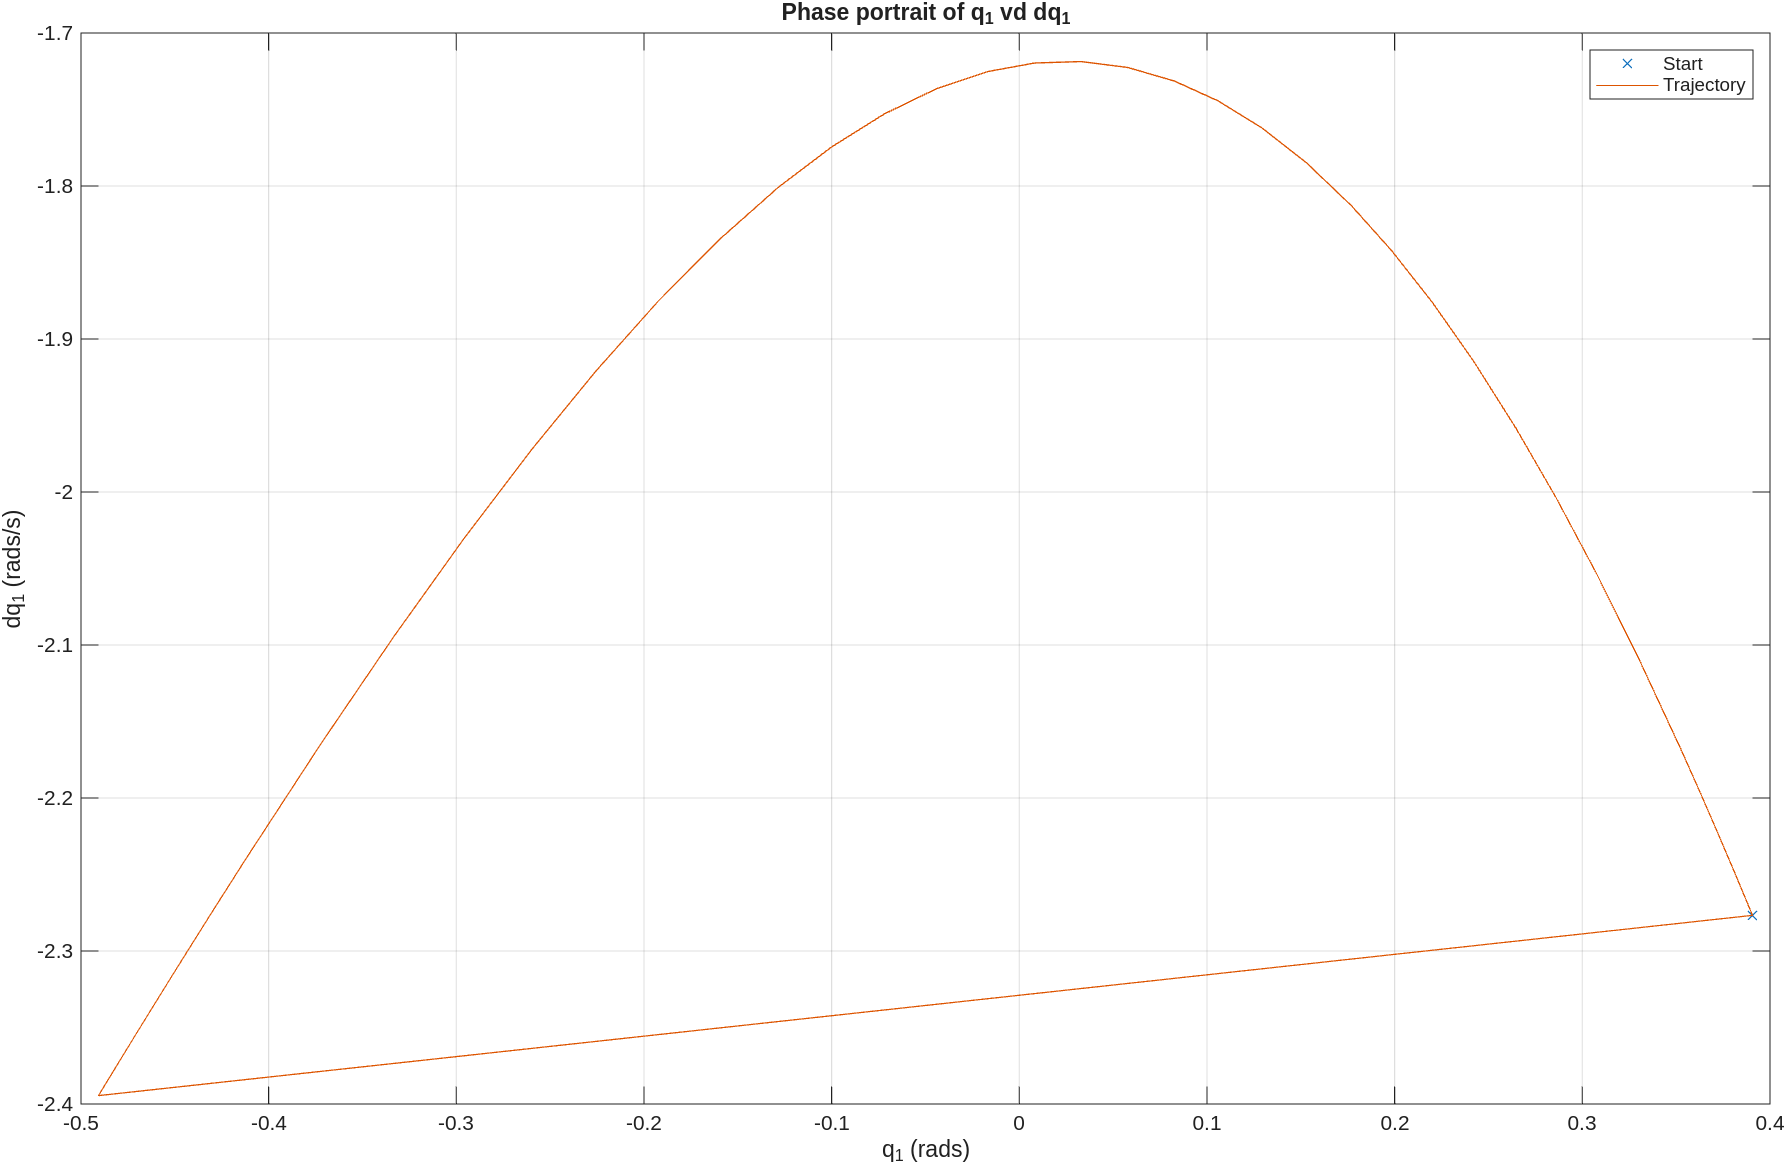
\includegraphics[width=0.8\textwidth]{ZD.png}
    \caption{Phase portrait of the zero dynamics ($q_1$ vs.\ $\dot{q}_1$).}
\end{figure}

\end{document}
